\documentclass{article}
\usepackage[utf8]{inputenc}

\title{Tutorial PNET Backend}
\author{Guillermo López García, Elías Makdad}
\date{\today}

\usepackage{natbib}
\usepackage{graphicx}
\usepackage{url}
\usepackage{listings}
\usepackage{float}

\begin{document}

\maketitle

\tableofcontents

\section{Introduction}
En este tutorial vamos a explicar paso por paso como hemos desarrollado todo el backend y como arrancarlo de forma sencilla una vez puesto.
Por otra parte, también explicaremos como hemos creado la base de datos en heroku.

\section{NPM}
Bien, lo primero que debemos tener en cuenta a la hora de iniciar un proyecto con las tecnologías de NodeJS es que vamos a trabajar con NPM. NPM es el gestor de librerías más famoso de JavasScript, aunque no el único (también existe Yarn).

Por ende, lo primero que vamos a hacer es iniciar un proyecto con NPM. Por ende, debemos instalar previamente en nuestro equipo NPM.

Según como sea nuestro sistema, Windows o Linux, lo haremos basandonos en esta guía de la propia web de NPM \url{https://www.npmjs.com/get-npm}.

Una vez instalado, abriremos una consola de comandos, y escribiremos en el directorio que deseemos el comando:
\begin{lstlisting}[language=bash]
  $ npm init
\end{lstlisting}

Este comando nos pedira una serie de información sobre el proyecto, tales como el autor o el archivo main a ejecutar.

Nosotros lo hemos hecho dentro de la carpeta llamada principal en nuestro directorio de proyeto, poniendo como archivo main el archivo con la ruta 'backend/index.js'.

Así pues, con el comando:
\begin{lstlisting}[language=bash]
  $ node .
\end{lstlisting}
se iniciaría directamente el archivo 'backend/index.js', sin tener que especificar la ruta del mismo.

Por otra parte, para instalar todas las dependencias exigidas, nos movemos a la raíz del proyecto y ejecutamos: 
\begin{lstlisting}[language=bash]
  $ npm install
\end{lstlisting}
Así ejecutamos la instalación de todas las dependencias del proyecto.

Queda aclarar que dicho comando se basa en el archivo 'package.json', que en nuestro proyecto tiene la siguiente información:

\begin{lstlisting}[language=bash]
{
  "name": "pnet",
  "version": "1.0.0",
  "description": "Repositorio para la asignatura Programación en Internet",
  "main": "backend/index.js",
  "dependencies": {
    "cors": "^2.8.5",
    "express": "^4.17.1",
    "html5-validator": "^1.2.1",
    "mongodb": "^3.5.5",
    "morgan": "^1.10.0"
  },
  "devDependencies": {},
  "scripts": {
    "test": "echo \"Error: no test specified\" && exit 1"
  },
  "repository": {
    "type": "git",
    "url": "git+https://github.com/guilogar/pnet.git"
  },
  "author": "",
  "license": "ISC",
  "bugs": {
    "url": "https://github.com/guilogar/pnet/issues"
  },
  "homepage": "https://github.com/guilogar/pnet#readme"
}
\end{lstlisting}

\section{Heroku y Database MongoDB}
En este paso, explicaremos como crear una cuenta en Heroku y crear dentro de ella una base de datos MongoDB para proveernos servicio de persistencia de datos.

En primer lugar, nos debemos crear una cuenta gratuita en \url{heroku.com}. La forma de crearse una cuenta en dicho sitio web es trivial, así no adjuntamos captura.

Pero, una vez nos registremos, ya podemos empezar a crear un proyecto donde adjuntaremos nuestra base de datos.

Así pues:

\begin{figure}[H]
\centering
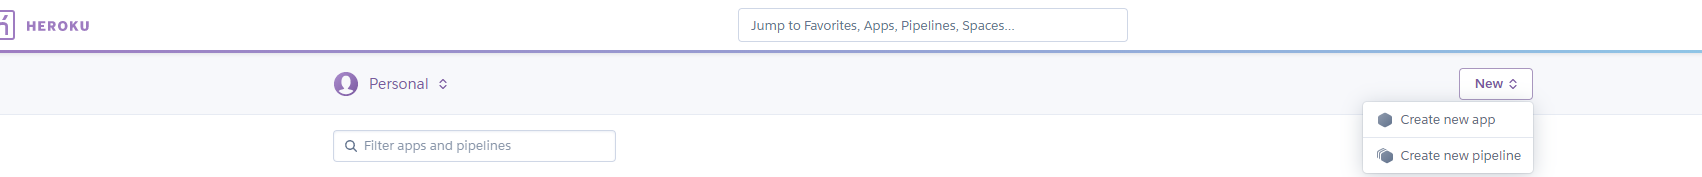
\includegraphics[width=\textwidth]{heroku/new_project1}
\caption{New project heroku}
\label{fig:universe}
\end{figure}

\begin{figure}[H]
\centering
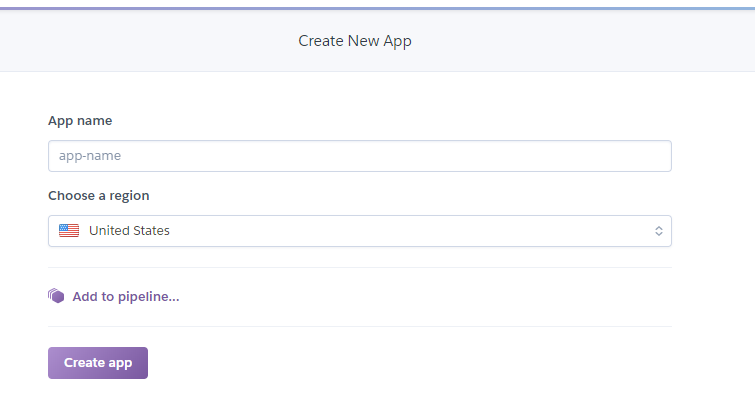
\includegraphics[width=\textwidth]{heroku/new_project2}
\caption{New project heroku}
\label{fig:universe}
\end{figure}

\begin{figure}[H]
\centering
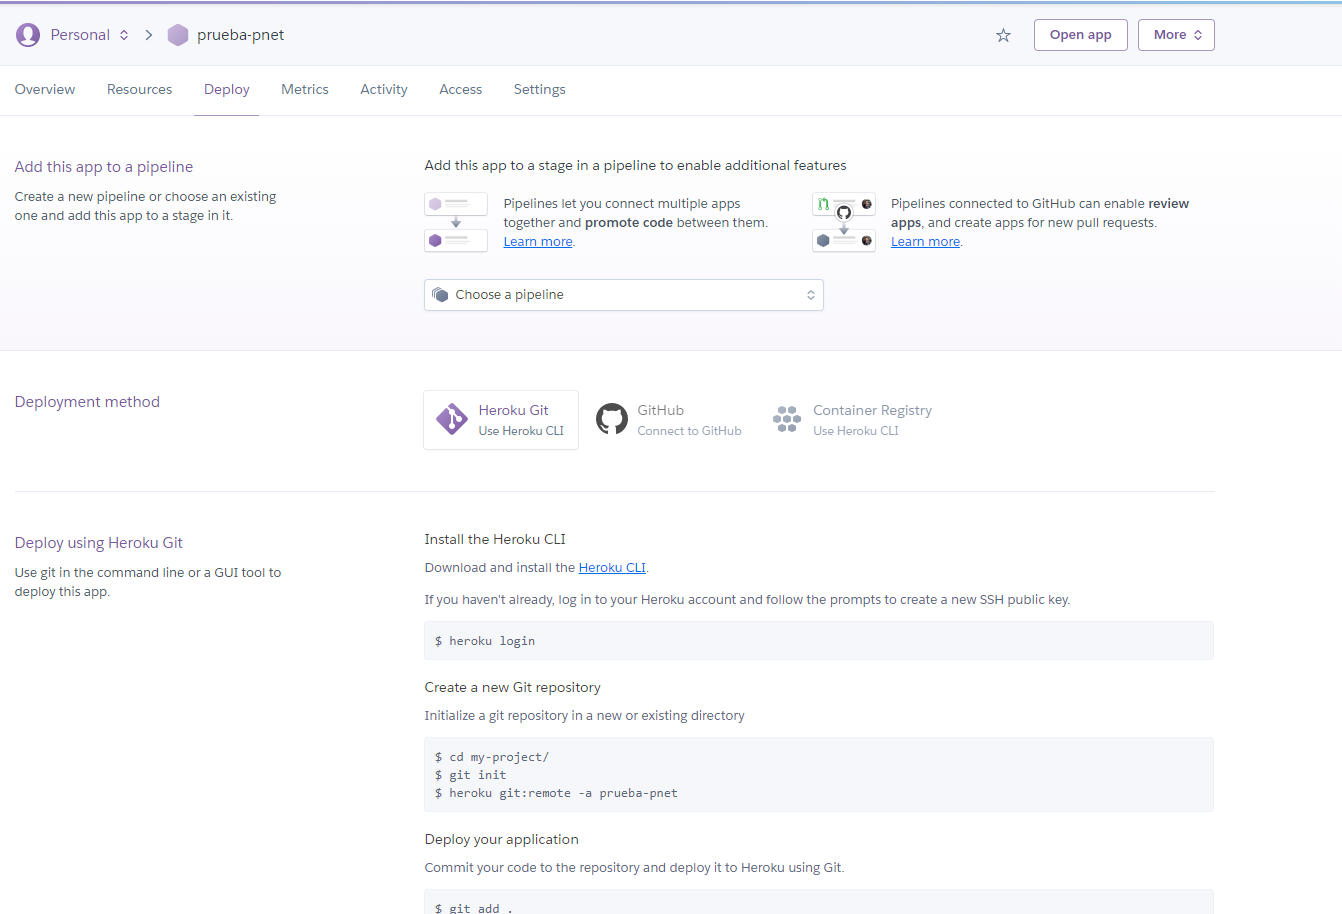
\includegraphics[width=\textwidth]{heroku/new_project3}
\caption{New project heroku}
\label{fig:universe}
\end{figure}

\begin{figure}[H]
\centering
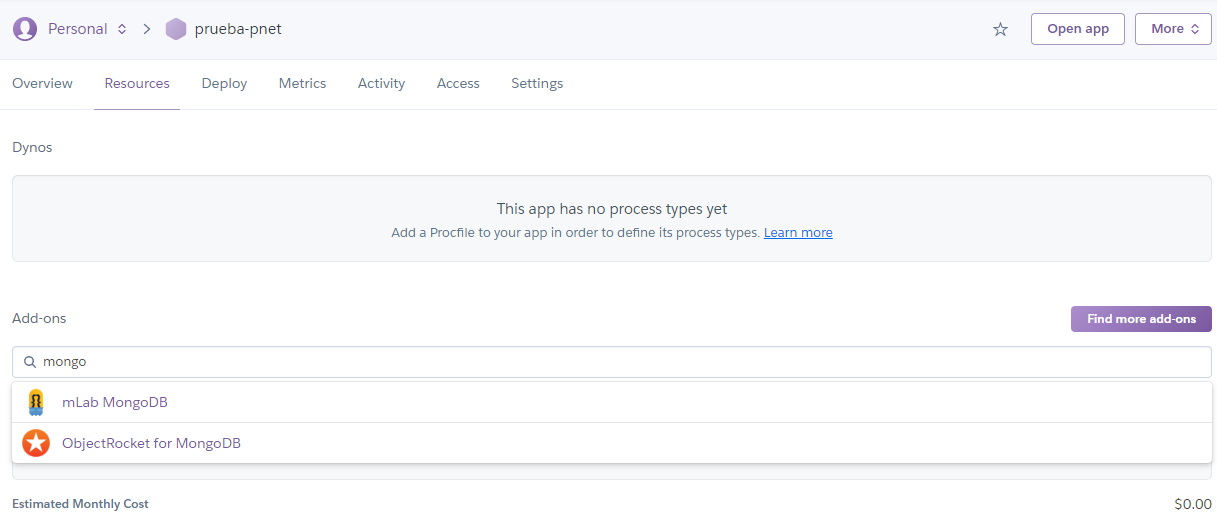
\includegraphics[width=\textwidth]{heroku/new_project4}
\caption{New project heroku}
\label{fig:universe}
\end{figure}

\begin{figure}[H]
\centering
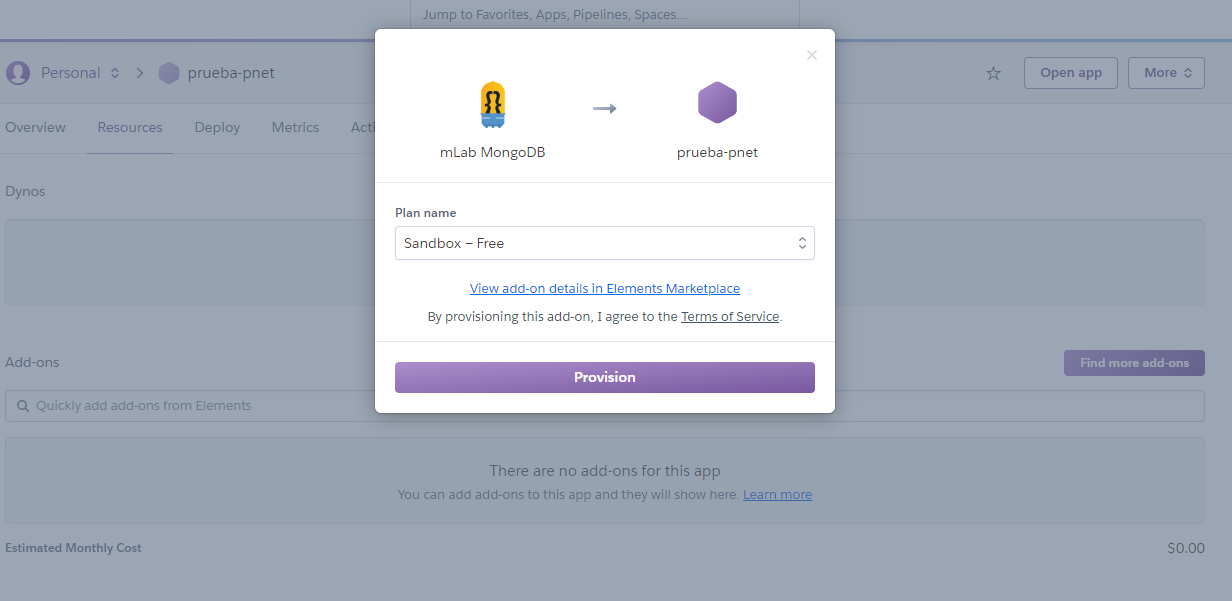
\includegraphics[width=\textwidth]{heroku/new_project5}
\caption{New project heroku}
\label{fig:universe}
\end{figure}

\begin{figure}[H]
\centering
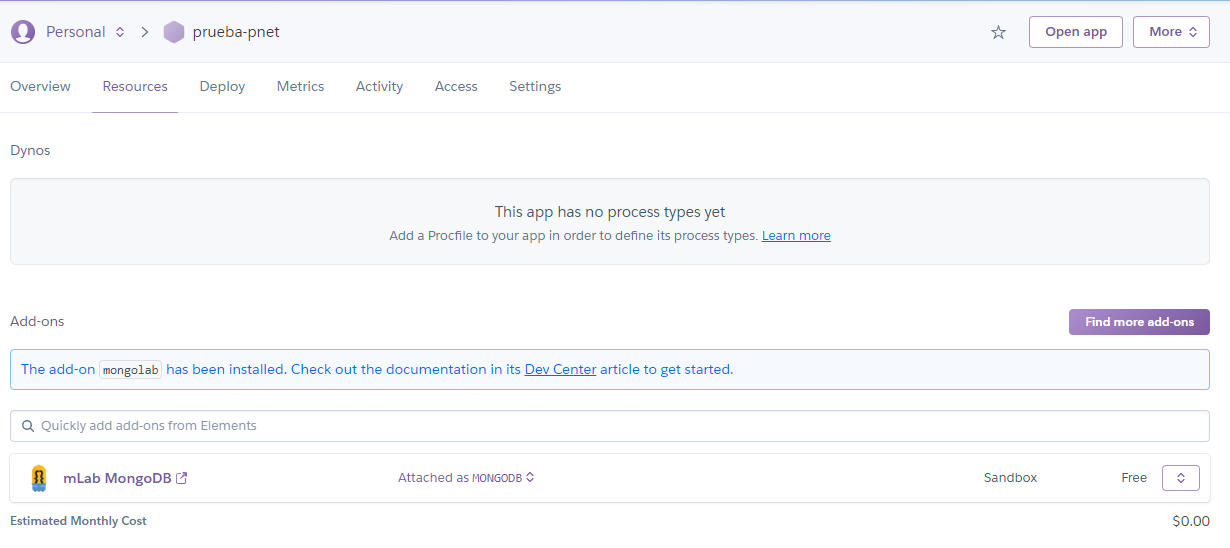
\includegraphics[width=\textwidth]{heroku/new_project6}
\caption{New project heroku}
\label{fig:universe}
\end{figure}

\begin{figure}[H]
\centering
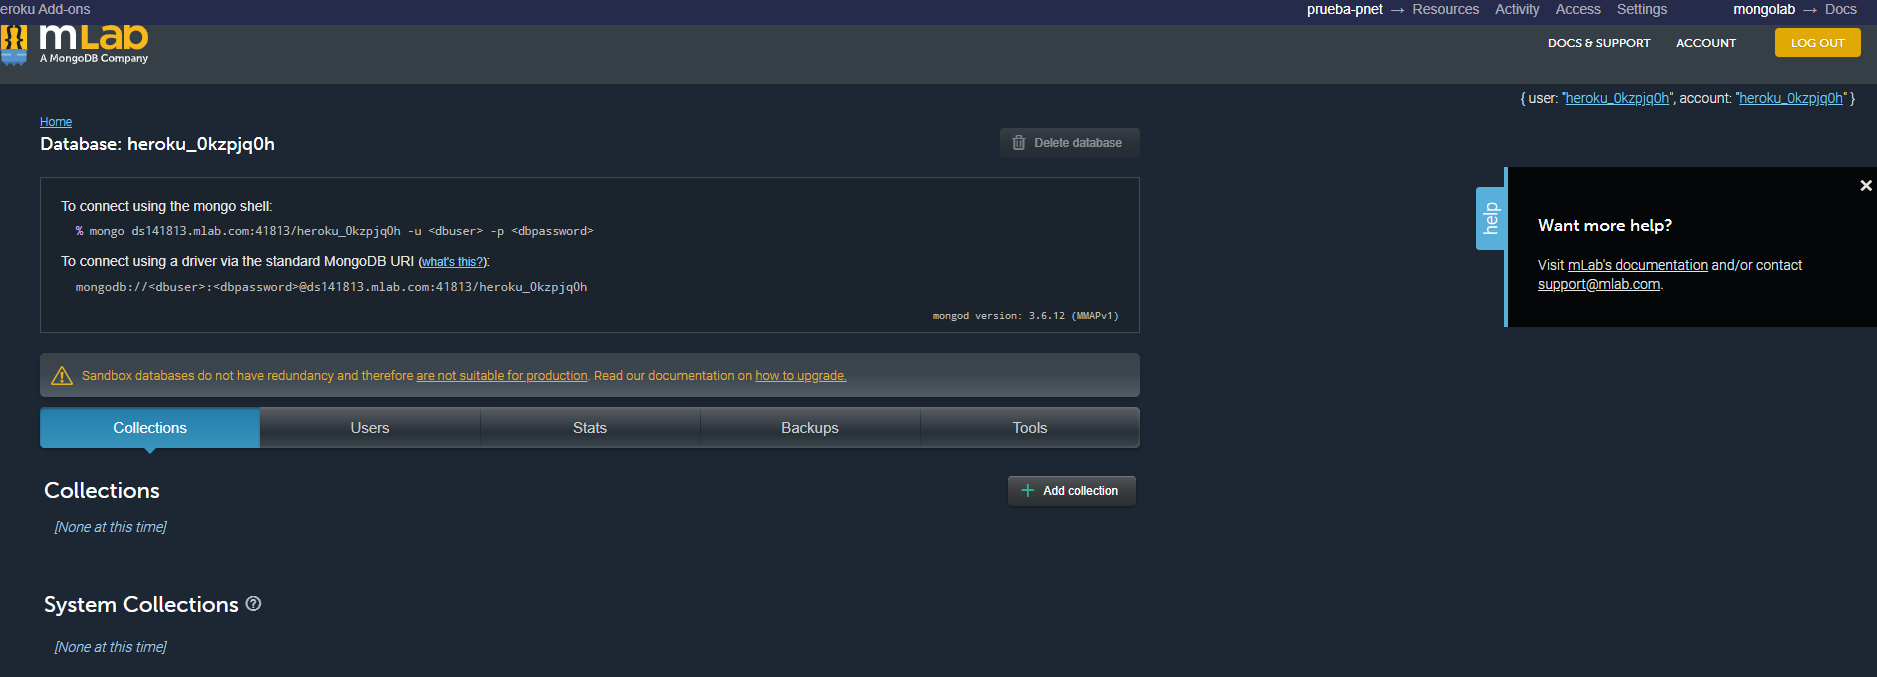
\includegraphics[width=\textwidth]{heroku/new_project7}
\caption{New project heroku}
\label{fig:universe}
\end{figure}

Bien, una vez creado el proyecto y con las credenciales de la base de datos MongoDB obtenida, ya podemos empezar a trabajar en el siguiente paso.

\section{DatabaseService MongoDB}
Bien, en este paso, explicaremos como se ha creado un servicio parametrizable para acceder a la base de datos MongoDB existente en Heroku.

A continuación, exponemos el código y explicamos el porqué del mismo.

\begin{lstlisting}[language=C++]
'use strict';

const MongoClient = require('mongodb').MongoClient;

const ObjectId = require('mongodb').ObjectID;

const USERNAME = 'pnet-guillermo-elias';
const PASSWORD = 'pnet-guillermo-elias3000';

class Database {
    async connectDb (callback, collectionDatabase)
    {
        try
        {
            const database = await MongoClient.connect(
                "mongodb://" + USERNAME + ":" + PASSWORD +
                "@ds157834.mlab.com:57834/heroku_0dql66zr",
                { useNewUrlParser: true, useUnifiedTopology: true }
            );
            this.database = database;
            this.db = 
                await database
                .db('heroku_0dql66zr')
                .collection(collectionDatabase);
            return this.db;
        } catch(err)
        {
            callback(err);
        }
    }

    async add (object, callback) {
        return await this.db.insertOne(object, callback);
    };

    async get (_id, callback) {
        return await 
            this.db
            .find({_id: ObjectId(_id)}).toArray(callback);
    };
    
    async getAll (callback) {
        return await this.db.find({}).toArray(callback);
    };
    
    async update (_id, updatedObject, callback) {
        delete updatedObject._id;
        return await 
            this.db
            .updateOne(
                {_id: ObjectId(_id)},
                {$set: updatedObject},
                callback
            );
    };
    
    async remove (_id, callback) {
        return await
            this.db
            .deleteOne(
                {_id: ObjectId(_id)},
                callback
            );
    };
    
    async removeAll (callback) {
        return await this.db.deleteMany({}, callback);
    };

    async close() {
        try
        {
            this.database.close();
        } catch(err) {
            console.log(err)
        }
    }
};

module.exports.Database = Database;
\end{lstlisting}

Como se puede apreciar en la lectura del código fuente, el acceso a la base de datos se ha convertido en una clase parametrizable, con el objetivo de que si más adelante tenemos que cambiar el acceso a la base de datos por otra que no sea MongoDB, tendriamos que modificar muchas partes del código para efectuar dicho cambio.

A parte, se ha encapsulado dentro de una clase en una lugar de una función para mayor legibilidad.

Además, se ha utilizado el sistema de programación 'async - await' que nos proporciona JavaScript de forma nativa, pudiendo hacer procesamiento de forma asíncrona y no basado en callbacks (forma anticuada de programar en JavaScript).

Como último dato a comentar de este código, es que el método connectDb recibe un 'callback' y un parametro llamado 'collectionDatabase'. El segundo es utilizado para definir a que colección de la base de datos de MongoDB queremos operar. El primero, se usa para pasar un 'callback'. Pero no es una contradicción con lo que he escrito antes, ya que, con excepciones, se pueden usar los 'callbacks'. Leasé \url{https://developer.mozilla.org/es/docs/Glossary/Callback_function}.

Bien, una vez parametrizada el acceso a la base de datos, procedemos a explicar el siguiente paso.

\section{Routers}
Bien, una vez explicado y entendido todo lo anterior, procedemos a la creación de Routers. Es un recurso bastante empleado en NodeJS.

Para facilitar la comprensión del mismo, pasamos a exponer el código y luego explicar el porqué del mismo.

Así pues:

\begin{lstlisting}[language=C++]
'use strict';

const express = require('express');
const router = express.Router();
const { Database } = require('./database-service');
const databaseServiceNotifications = new Database();

databaseServiceNotifications.connectDb(
    function(err)
    {
        if (err)
        {
            console.log(
            'Could not connect with MongoDB ' + 
            '– databaseServiceNotifications',
            err
            );
            process.exit(1);
        }
    }, 'notifications'
);

router.get('/notifications', function (req, res) {
	databaseServiceNotifications.getAll((err, object) => {
            if (err) {
                res.status(500).send({
                    msg: err
                });
            } else if (object === null){
            	res.status(500).send({
                    msg: "object null"
                });
            } else {
                res.status(200).send(object);
            }
        }
    );
});

router.post('/notifications', function (req, res) {
    let object = req.body;
    databaseServiceNotifications.add(object, (err, object) => {
            if (err) {
                res.status(500).send({
                    msg: err
                });
            } else if (object !== null) {
                res.status(201).send({
                    msg: 'object created!'
                });
            }
        }
    );
});

router.delete('/notifications', function (req, res) {
    databaseServiceNotifications.removeAll((err) => {
        if (err) {
            res.status(500).send({
                msg: err
            });
        } else {
            res.status(200).send({
                msg: 'object deleted!'
            });
        }
    });
});

router.get('/notifications/:_id', function (req, res) {
    let _id = req.params._id;
    databaseServiceNotifications.get(_id, (err, object) => {
        if (err) {
            res.status(500).send({
                msg: err
            });
        } else if (object === null){
            res.status(500).send({
                msg: "object null"
            });
        } else {
            res.status(200).send(object);
        }
    });
});

router.put('/notifications/:_id', function (req, res) {
    const _id = req.params._id;
    const updatedobject = req.body;
    databaseServiceNotifications
        .update(_id, updatedobject, (err, numUpdates) => {
        if (err || numUpdates === 0) {
            res.status(500).send({
                msg: err
            });
        } else {
            res.status(200).send({
                msg: 'object updated!'
            });
        }
    });
});

router.delete('/notifications/:_id', function (req, res) {
    let _id = req.params._id;
    databaseServiceNotifications.remove(_id, (err) => {
        if (err) {
            res.status(404).send({
                msg: err
            });
        } else {
            res.status(200).send({
                msg: 'object deleted!'
            });
        }
    });
});

module.exports = router;
\end{lstlisting}

Bien, como se puede apreciar en dicho código, lo primero que hacemos a parte de inicializar el objeto Router de la librería NodeJS, es inicializar la conexión hacia la base de datos (clase Database) con los parametros necesitados por nosotros en este caso en concreto.

Como se puede apreciar, le indicamos la colección 'notifications' como la colección con la que queremos trabajar. También, le pasamos en primera instancia una función 'callback' para mostrar un error personalizado en caso de que la conexión a la base de datos fallé.

Bien, una vez realizada la conexión con la base de datos correctamente, solo queda la creación de los routers indicando las url de los endpoints por los que escucharemos las peticiones entrantes y que código de servidor ejecutaremos. Al utilizar sobre el objeto 'router' los métodos 'get', 'post', 'put' y 'delete', indicamos que la cabecera de la petición ha de tener el método indicado para cada acción que queramos realizar frente al servidor.

Este ejemplo, esta basado sobre una entidad llamada 'notifications', guardada como colección dentro de la base de datos MongoDB.

Bien, una vez entendido el código anterior, pasamos a explicar el siguiente paso.

\section{Arrancar el servidor - index.js}
Bien, ya solo nos queda arrancar el servidor y empezar a realizar las acciones que nos pidan según el endpoint pedido.

Como se ha hecho a lo largo de este tutorial, expondremos el código y posteriormente, explicaremos el porqué del mismo.

Así pues:

\begin{lstlisting}[language=C++]
const express = require('express');
const app = express();
const logger = require('morgan');
const http = require('http');
const path = require('path');
const PORT = process.env.PORT || 3000;
const bodyParser = require('body-parser');
const baseAPI = '/api/v1';
const cors = require('cors');

app.use(cors()); // For enable cors
app.use(bodyParser.json()); // For enable json parse always
app.use(logger('dev'));
app.use(bodyParser.urlencoded({
    extended: true
}));

const timetable = require('./routes/timetable');
const inscriptions = require('./routes/inscriptions');
const speakers = require('./routes/speakers');
const notifications = require('./routes/notifications');

app.use(baseAPI, timetable);
app.use(baseAPI, inscriptions);
app.use(baseAPI, speakers);
app.use(baseAPI, notifications);

const server = http.createServer(app);

server.listen(PORT, function() {
    console.log('Server up and running on localhost:' + PORT);
});
\end{lstlisting}

Como podemos observar, el archivo 'index.js' es bastante corto, ya que, el resto del código esta lo suficientemente modulado y parametrizado como para no tener que repetir código.

Como se puede observar también, tan solo se invocan los routers, pero no el servicio de la base de datos, ya que, cada router se encarga se inicializar el acceso a su base de datos en caso de que lo necesite.

\section{Obtener datos de los Endpoint con el navegador (chrome, firefox, etc)}
Bien, una vez creado el servidor, e iniciado el mismo con el comando:

\begin{lstlisting}[language=bash]
    $ node .
\end{lstlisting}

Procedemos a obtener datos del mismo. Para hacer esto, podemos usar un navegador mismo. En concreto, en este ejemplo, se ha usado chrome.

Bien, para interactuar con la api que esta en el servidor de NodeJS escuchando, es tan facil como acceder al localhost por el puerto especificado y el endpoint deseado.

En concreto, en el ejemplo que se va a mostrar en la imagen, hemos accedido a la parte de la api que nos proporciona un listado completo de los todos los objetos de la colección 'notifications'.

Así pues:

\begin{figure}[H]
\centering
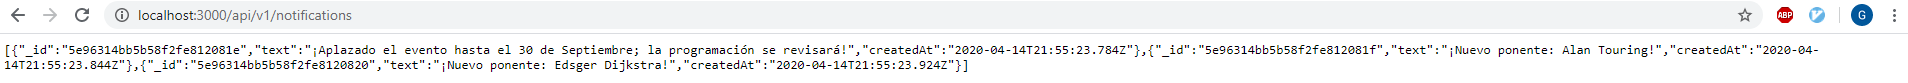
\includegraphics[width=\textwidth]{api/get_data_api}
\caption{Obteniendo datos de la Api con el navegador}
\label{fig:universe}
\end{figure}

Para interactuar con los métodos POST, PUT y DELETE ya sería necesario usar programación o bien, un cliente especifico como POSTMAN. En concreto, nosotros, hemos empleado la programación con jQuery, como vamos a explicar en el siguiente paso.

\section{Obtener datos de los Endpoint con programación de jQuery}
Bien, para este paso, vamos a exponer el código fuente, y a explicar el porqué del mismo.

\begin{lstlisting}[language=C++]
// IMPORTANT: in all code, i use the method append of
// jquery for add the elements.
// For more information, see https://api.jquery.com/append/
const notificationsUrl = "http://localhost:3000/api/v1/notifications";
$.ajax({
    type: "GET",
    dataType: "json",
    url: notificationsUrl,
    success: function(data)
    {
        $('aside.news-body').empty();
        $('aside.news-body').hide();
        // iterate notifications...
        for(const notification of data)
        {
            // create the article....
            let article = 
                $('<article class="alert alert-secondary"></article>');
            let span = $('<span class="header-news-body"></span>');
            span.text(notification.text);
            article.append(span);
            let button = 
                $('<button type="button" class="close" data-dismiss="alert"' + 
                  'aria-label="Close"><span aria-hidden="true">&times;</span>' +
                  '</button>');
            article.append(button);
            $('aside.news-body').append(article);
        }
        $('aside.news-body').slideDown('slow');
    },
    error: function(err)
    {
        console.log(err);
    }
});
\end{lstlisting}

Como se puede apreciar en este código, es una clásica sección de código para obtener datos de un servidor y posteriormente, inscrustarlo en la página web mediante generación de código dinámico.

En concreto, para generar los elementos se ha usado jQuery y para los estilos de los mismo, se ha usado Bootstrap 4.0.

\begin{thebibliography}{9}
\bibitem{mozilla} 
JavaScript documentation,
\\\texttt{https://developer.mozilla.org/es/docs/Web/JavaScript}

\bibitem{nodejs} 
NodeJS documentation,
\\\texttt{https://nodejs.org/es/docs/}

\bibitem{mongodb} 
MongoDB documentation,
\\\texttt{https://docs.mongodb.com/manual/}

\bibitem{bootstrap} 
BootStrap documentation,
\\\texttt{https://getbootstrap.com/docs/4.4/getting-started/introduction/}

\bibitem{fontawesome} 
FontAwesome documentation,
\\\texttt{https://fontawesome.com/how-to-use/on-the-web/referencing-icons/basic-use}
\end{thebibliography}
\end{document}